\chapter{Situation}

\begin{rpg-commentbox}{Overview}
    Melting Point is a complete cinematic scenario for Alien roleplaying game. The intention is that the scenario can be played from two different perspectives: corporate crew \& prisoners. In the current draft, I focus on prisoners.
\end{rpg-commentbox}


\section{Scenario Overview}

The setup is quite straightforward: Weyland-Yutani Kohru, lithium refinery station operates under United Americas surveillance. 
The corporation provides technical knowhow while the government provides labor force in the form of captured terrorists. 

Many of the prisoners at Kohru had never faced trial or charges, they were caught under the United America terrorist act. Lack of communication, time for lawyers to travel to the place at the edge of the charted systems, and all the corporate bureaucracy has made the location a living nightmare.  



The station operates on a cryosleep round robin algorithm, i.e., to avoid riots only a handful prisoners are awake at any given time. Other cryosleep chambers are heavily protected and out of limits. At each round robin rotation, a synthetic is put alongside the prisoners so that it can gather data about potential terrorist attacks, evidence, and information for blackmailing purposes.


Weapons and tooling at the location work either with biometric fingerprints or geo-location. For instance, a prisoner cannot light a welding torch near elevator entrances, but can do so in the refinery. As another example, only security staff can fire pistols due to biometric locks.


When a not so standard inspection occurs, hell cuts lose and the station enters quarantine lock-down putting prisoners and wardens against each other.
What will the station crew do? Will the prisoners ally or will old grudges turn them one against the others? 





\medskip
\begin{rpg-commentbox}{Science Background}
\begin{small}
\textit{Lithium is a highly reactive alkali metal that offers excellent heat and electrical conductivity.  These properties make it particularly useful for the manufacture of glass, high-temperature lubricants, chemicals, pharmaceuticals, and lithium ion batteries for electric cars and consumer electronics}

\textit{The process for recovering lithium from ore can vary based on the specific mineral deposit in question. In general, the process entails removing the mineral material from the earth then heating and pulverizing it. The crushed mineral powder is combined with chemical reactants, such as sulfuric acid, then the slurry is heated, filtered, and concentrated through an evaporation process to form salable lithium carbonate, while the resulting wastewater is treated for reuse or disposal.}    
\end{small}
\end{rpg-commentbox}



\medskip
\begin{rpg-commentbox}{Setting game difficulty}
\begin{itemize}
    \item \textbf{Normal}: as described in the booklet;
    \item \textbf{Hard}: non-lethal weapons only, e.g., shotguns fire rubber bullets;
\end{itemize}
\end{rpg-commentbox}

\newsect

\newpage

\begin{sidewaysfigure*}
    \centering
    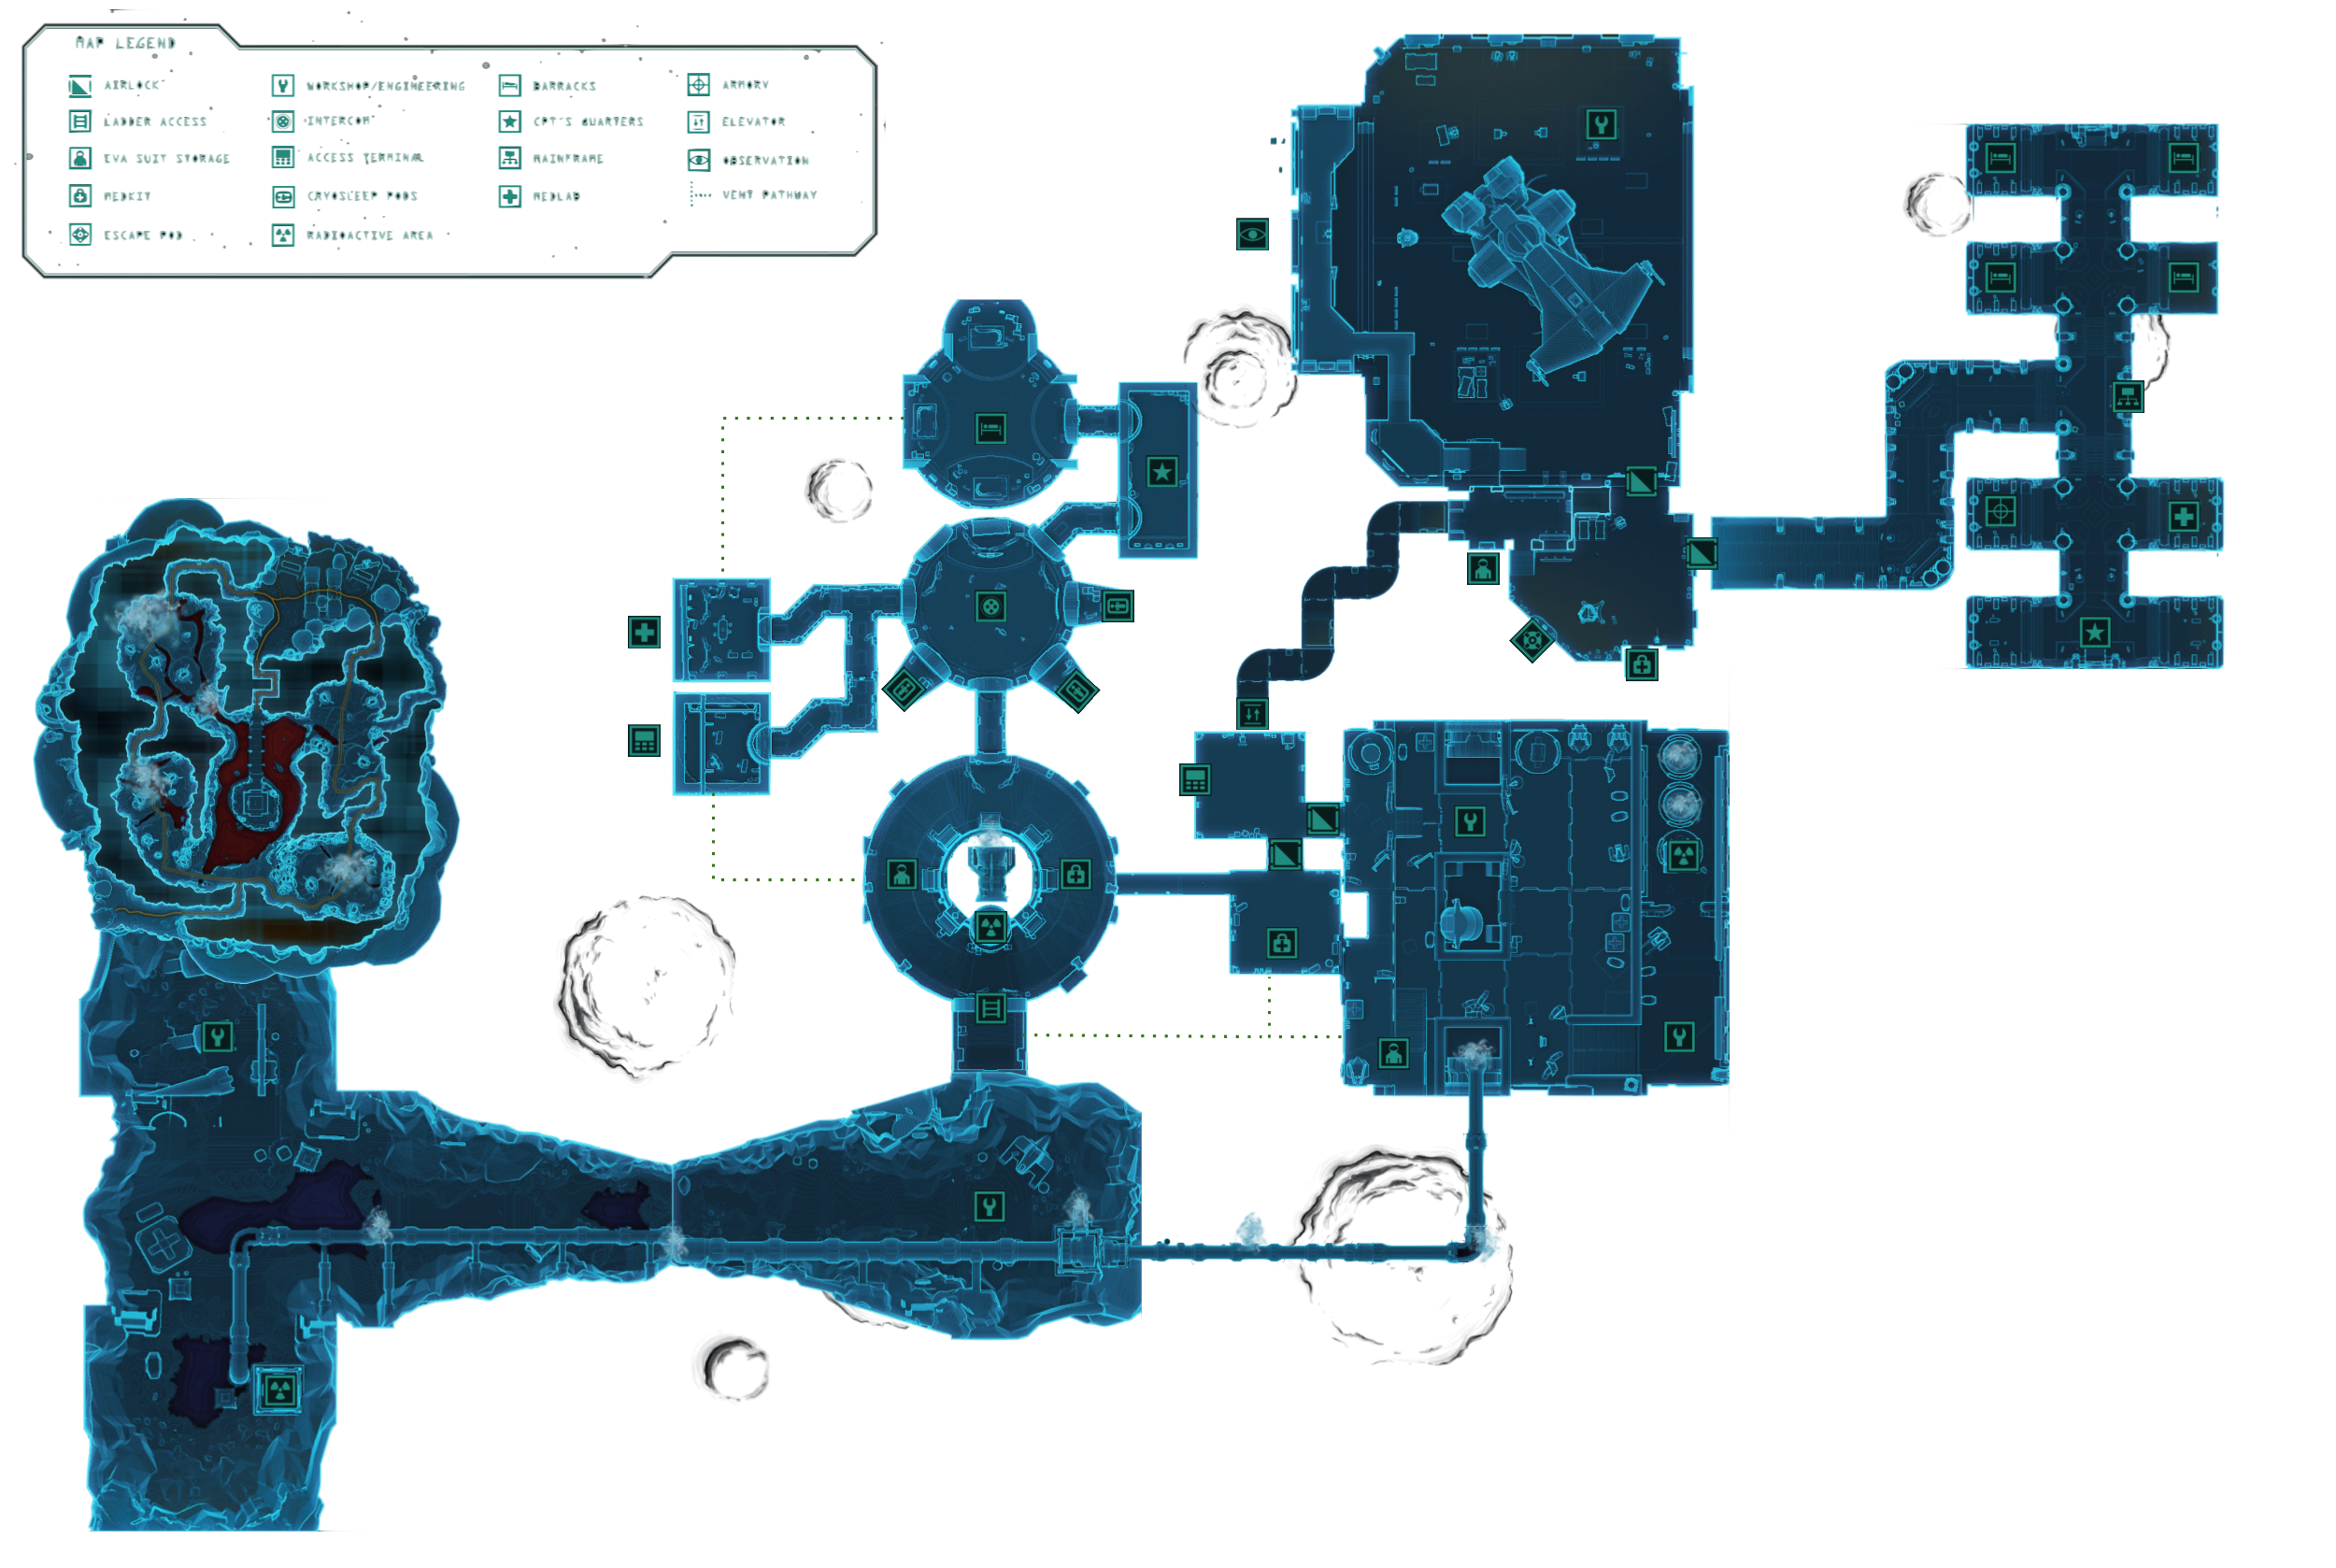
\includegraphics[width=1.05\textwidth]{img/space-refinery-final.png}
    \label{fig:refinery}
\end{sidewaysfigure*}

\newpage